% 
% Annual Cognitive Science Conference
% Sample LaTeX Paper -- Proceedings Format
% 

% Original : Ashwin Ram (ashwin@cc.gatech.edu)       04/01/1994
% Modified : Johanna Moore (jmoore@cs.pitt.edu)      03/17/1995
% Modified : David Noelle (noelle@ucsd.edu)          03/15/1996
% Modified : Pat Langley (langley@cs.stanford.edu)   01/26/1997
% Latex2e corrections by Ramin Charles Nakisa        01/28/1997 
% Modified : Tina Eliassi-Rad (eliassi@cs.wisc.edu)  01/31/1998
% Modified : Trisha Yannuzzi (trisha@ircs.upenn.edu) 12/28/1999 (in process)
% Modified : Mary Ellen Foster (M.E.Foster@ed.ac.uk) 12/11/2000
% Modified : Ken Forbus                              01/23/2004
% Modified : Eli M. Silk (esilk@pitt.edu)            05/24/2005
% Modified : Niels Taatgen (taatgen@cmu.edu)         10/24/2006
% Modified : David Noelle (dnoelle@ucmerced.edu)     11/19/2014

%% Change "letterpaper" in the following line to "a4paper" if you must.

\documentclass[10pt,letterpaper]{article}

\usepackage{cogsci}
\usepackage{pslatex}
\usepackage{apacite}

\usepackage{amsmath}
\usepackage{graphicx}
\usepackage{subcaption}

% http://tex.stackexchange.com/questions/205342/issues-with-flushend-last-citation-cut-etc 
\usepackage[keeplastbox]{flushend}  % balance the final columns

\renewcommand{\vec}[1]{{\bf {#1}}}
\newcommand{\dotp}[3]{\left\langle {#1}, {#2} \right\rangle_{#3}}
\newcommand{\lif}[2]{G_{#1} \left[ {#2} \right]}

\title{A spiking neural model for learning priors}
 
\author{{\large \bf Sugandha Sharma (s72sharm@uwaterloo.ca)} \\
  {\large \bf Chris Eliasmith (celiasmith@uwaterloo.ca)} \\
  Centre for Theoretical Neuroscience, University of Waterloo \\
  Waterloo, ON, Canada, N2L 3G1}


\begin{document}

\maketitle

\begin{abstract}
In this paper, we present a spiking neural model of learning priors for a lifespan inference task. Through this model, we extend our previous work on the biological plausibility of performing Bayesian computations in the brain. Specifically, we address the 
question of how humans might be generating the priors needed for this inference. We propose neural mechanisms that may be involved in continuous learning and updating of priors and may be applicable in many aspects of higher-level cognition. We show that the model is generalizable and is able to converge to the near optimal priors with very few training samples. 

\textbf{Keywords:} 
neural engineering; computational neuroscience; expectation maximization; bayesian inference
\end{abstract}

\section{Introduction}

The Bayesian framework has successfully described performance in many cognitive tasks where sensory information is combined with prior assumptions. It has also been shown that the prior knowledge of statistical regularities in the environment allows humans to make accurate estimations. For example~\citeA{griffiths2006optimal} asked people to make predictions about the duration or extent of everyday phenomena such as human life spans or the box-office earnings of movies, and showed a close correspondence between people’s implicit probabilistic models and the statistics of the world. 

However, whether these priors are hard-wired or learned in response to environmental statistics is the subject of debate. A human infant is born with some biological capacities for learning that are then realized by the environment surrounding a newborn. For example, it is generally agreed that newborns have an inherent sense of motion, space, numbers, and can distinguish animate from inanimate objects~\cite{spelke2007core}, ~\cite{izard2009newborn}. However, the environment surrounding a newborn also supplies structured information that assists in actualizing their raw capacities. Thus learning seems to be promoted by both the child's biology and its' environment. It is thus plausible that some cortical areas represent hypotheses (sometimes learned, sometimes innate) regarding the properties of the world, which are used to interpret complex and ambiguous sensory input.

%While it's not clear exactly how much knowledge is there at the beginning, we can see the mind as having hypothesis about how the world works. In other words, some cortical areas in the brain might represent hypothesis regarding the properties of the world, which could be used to interpret complex and ambiguous sensory input.

We have previously shown how Bayesian computations combining a hypothesis with sensory input may be implemented in a biologically plausible neural network. Specifically, we presented a method for representing probability distributions using neural circuits and combining them in meaningful ways to perform inference~\cite{sharma2017}. However, the prior used for inference was obtained empirically, and externally to the model. In this paper, we extend our neural model to explore how the priors might be learned in the human brain. Specifically, we show how priors can be learned from life experience and how this learning process could be directed by the existing hypotheses in the brain. The resultant neural mechanisms for learning priors are not specific to a particular task, but can generalize to different tasks.

%-----------------------------------------------------------------------------
% How much knowledge is there at the beginning? How is knowledge represented? How is new knowledge learned?


\section{Background}

\subsection{Life span prediction task}

\citeA{griffiths2006optimal} evaluate how cognitive judgments compare with optimal statistical inference by asking people to predict human life spans. The responses were recorded and compared with the predictions made by a Bayesian model.

If $t_{total}$ indicates the total amount of time the person will live and $t$ indicates their current age, the task is to estimate $t_{total}$ from $t$. The Bayesian model computes a probability distribution over $t_{total}$ given $t$, by applying Bayes' rule:
\begin{equation}
\label{eqn:bayes_rule}
\begin{aligned}
p(t_{total} | t) = p(t | t_{total})p(t_{total}) / p(t) ,
\end{aligned}
\end{equation}
where:
\begin{equation}
\label{eqn:p_t}
\begin{aligned}
p(t) = \int_{0}^\infty p(t | t_{total})p(t_{total}) \, dt_{total} .
\end{aligned}
\end{equation}

Here, $p(t_{total})$ is the empirical prior distribution over life spans; $p(t | t_{total})$ is the probability of encountering a person at age $t$ given that their total life span is $t_{total}$ i.e., the likelihood. Assuming that we are equally likely to meet a person at any point in their life, this probability is uniform: 
\begin{equation}
\label{uniform_prob}
p(t | t_{total}) = 1/t_{total}, \text{ for $t < t_{total}$ (and 0 for $t \ge t_{total}$)}.
\end{equation}

 
\subsection{Neural model of life span inference}

In~\citeA{sharma2017}, we addressed the question of biological plausibility of Bayesian computations in the brain by presenting a neural model of lifespan inference task (described above) built using the Neural Engineering Framework~\cite<NEF;>{eliasmith2003neural}. There, we describe a method for representing high-dimensional distributions in neural circuits. Since probability distributions are most generally functions, we  approximate them as high-dimensional vectors over a fixed set of basis functions using the NEF. To do this, we define the relevant function domain by parameterizing the set of represented functions using an $n$-dimensional vector of coefficients $\vec{k} = \left[ k_1, k_2, \ldots, k_n \right]$ which define any function of interest over a fixed set of basis functions $\phi(\upsilon)$ as given below:
 
\begin{equation}
\label{eqn:function}
\begin{aligned} 
\vec{x}(\upsilon; \vec{k}) = \sum_{j=1}^n k_j \phi_j(\upsilon)   
\end{aligned}
\end{equation}

where \vec{x} is the subspace that is represented by the neurons.

Thus we exploit redundancy in function spaces by finding a basis space. This basis is used to project high-dimensional distributions on to a low-dimensional space by limiting the space spanned by the basis $\phi(\upsilon)$ to some subspace of interest (a particular probability distribution). The encoding and decoding functions used to compute connection weights are also projected to the low-dimensional space using the same basis. 

%Thus, we show the mathematical equivalence of (finite-dimensional) function spaces and (finite-dimensional) vector spaces.

Using these methods, we built a spiking neural model that is able to infer the total lifespan of an individual given their current age, and matches human performance on this task better than an ideal Bayesian model. This provides some evidence in support of the hypothesis that human brains represent low-dimensional
state spaces i.e., low-dimensional parameterizations of high dimensional
distributions fit using neural tuning curves. However, we used an empirical prior in this neural model. The question thus arises: How does our brain learn this prior? Next, we lay the theoretical groundwork for addressing this question and present a neural model that implements the proposed mechanism.

\section{Learning priors for generalized inference}

\begin{figure*}[ht]
\setlength{\belowcaptionskip}{-10pt}
\begin{center}
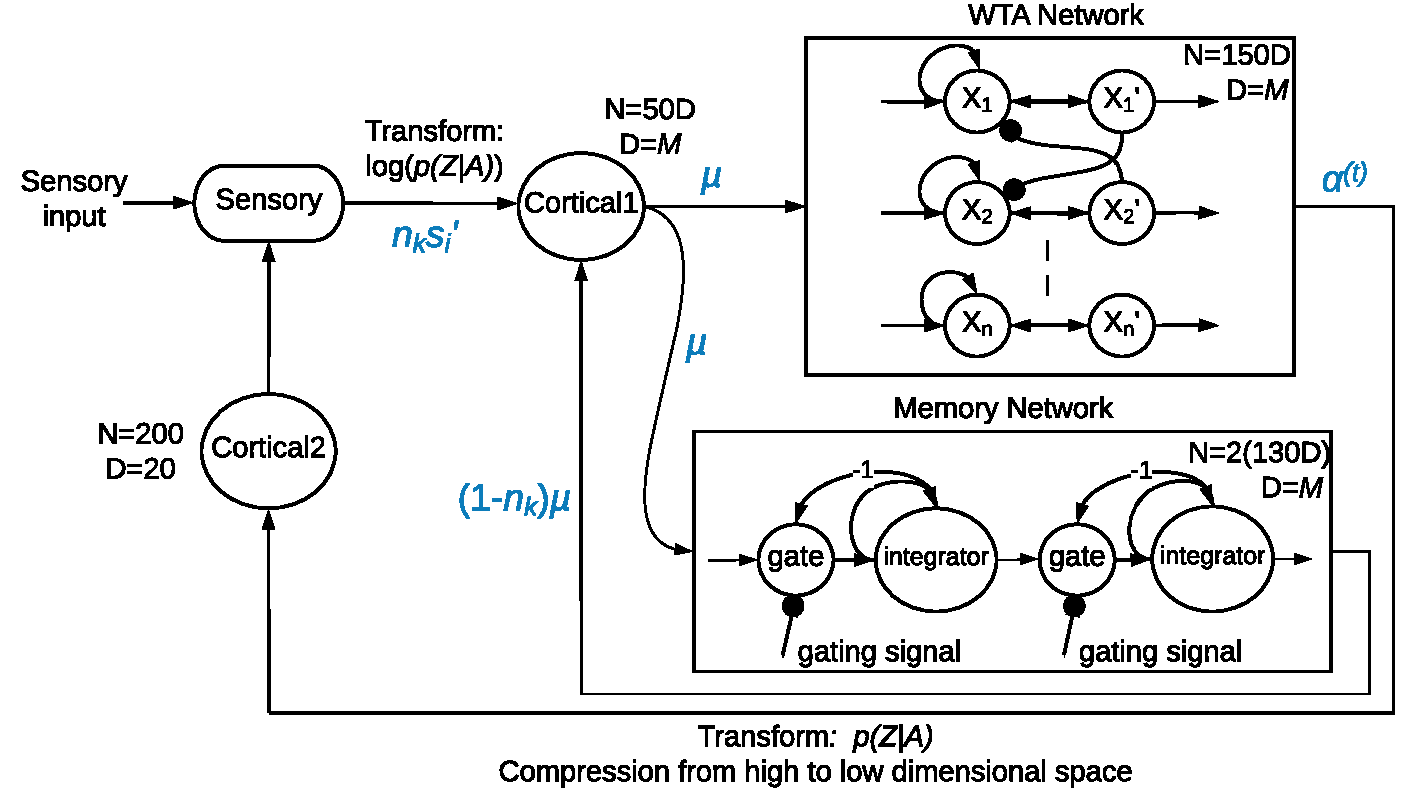
\includegraphics[width=0.70\linewidth,keepaspectratio]{model_schematic.pdf}
\end{center}
\caption{A schematic diagram of the neural model. The circles represent neural populations/networks. The rectangles group the neural populations into subnetworks. The rounded box represents a node (non-neural).  The flow of information is denoted with arrows ($\rightarrow$). Transformations are labelled along these connections. Inhibitory connections are indicated with full circles(---\textbullet). The blue labels indicate the quantity encoded by the spike trains propagating through the connections. The number of neurons and dimensions represented by each population/network are labelled as N and D respectively ($M$ is the prior space size).} 
\label{fig:model_schematic}
\end{figure*}


What neural mechanisms allow humans to learn the priors about life spans? We assume that humans learn the priors about life spans as a result of their life experience where they encounter people of different ages in their day to day lives. We further assume that the prior is parameterized by a set of unknown hyperparameters ($\alpha$) that are estimated from observed ages of $n$ distinct people, given by $\vec{X} = \{x_1, \ldots, x_n\}$. Here, each random variable $x_i$ corresponds to a separate $t$ from the previous model. Likewise, we model each element of $\vec{X}$ as being drawn independently from each element of $\vec{Z} = \{z_1, \ldots, z_n\}$ corresponding to the (unknown or hidden) life spans of these same $n$ people. Each random variable $z_i$ corresponds to a separate $t_{total}$ from the previous model, which in turn is drawn from the unknown prior. 

%In~\citeA{sharma2017}, we describe two standard methods for learning a prior by obtaining an estimate $\hat{\alpha}$ of the hyperparameters, which are briefly mentioned below, followed by the method that we adopt.

%We could directly find the hyperparameters $\hat{\alpha}$ that maximize the marginal likelihood of the observed data, $L(\alpha; \vec{X})$ (or equivalently the log-likelihood for numerical stability):
%\begin{equation}
%\label{eqn:marg_likelihood}
%\begin{split}
%L(\alpha; \vec{X}) &= p(\vec{X} | \alpha) = \prod_{i=1}^n p(x_i | \alpha) = \prod_{i=1}^n %\sum_{z_i} p(x_i, z_i | \alpha) \\
%\implies \: 
%\hat{\alpha} &= \text{argmax}_\alpha L(\alpha; \vec{X}) \\
%&= \text{argmax}_\alpha \log L(\alpha; \vec{X}) \\
%& = \text{argmax}_\alpha \sum_{i=1}^n \log \sum_{z_i} p(x_i, z_i | \alpha).
%\end{split}
%\end{equation}
%However, the procedure described above is intractable, since it requires that we iterate over all combinations of $\alpha$ and $\vec{Z}$. This motivates near-optimal iterative procedures such as the widely-used expectation maximization algorithm~\cite<EM;>{dempster1977maximum}. To begin, we simplify the expectation function using independence and other known facts about the model:

To estimate the hyperparameters $\hat{\alpha}$, we begin by writing the expectation function for the widely used Expectation Maximization algorithm~\cite<EM;>{dempster1977maximum}. 

\begin{equation}
\label{eqn:expectation_maximization}
\begin{aligned}
Q(\alpha | \alpha^{(t)}) &= E_{\vec{Z}|\vec{X},\alpha^{(t)}} \left[ \log L(\alpha; \vec{X}, \vec{Z}) \right] \\
&= \sum_{i=1}^n E_{z_i|x_i,\alpha^{(t)}} \left[ \log L(\alpha; x_i, z_i) \right] \\
&= \sum_{i=1}^n \sum_{z_i} p(z_i | x_i, \alpha^{(t)}) \log p(x_i, z_i | \alpha) \\
&= \sum_{i=1}^n \sum_{z_i} T(x_i, z_i) \log \left( p(x_i | z_i) p(z_i | \alpha) \right) \\
&= \sum_{i=1}^n \sum_{z_i} T(x_i, z_i) \log \left( p(z_i | \alpha) / z_i \right) ,
\end{aligned}
\end{equation}
where $\alpha^{(t)}$ is the current estimate for the hyperparameters obtained by maximizing the expectation with respect to the hyperparameters. We have defined $T(x_i, z_i) := p(z_i | x_i, \alpha^{(t)})$ to be some fixed function with respect to $\alpha^{(t)}$. The full derivation of the EM procedure for the lifespan inference task can be found in~\citeA{sharma2017}. 

This provides a tractable procedure for updating the prior. In particular, we begin with some initial guess at the hyperparameters, and then update them iteratively to better explain the observed data. However, each iteration in this procedure requires all observed ages of $n$ distinct people (Equation~\ref{eqn:expectation_maximization}). In other words, all observations $\vec{X} = \{x_1, \ldots, x_n\}$ are required to even begin learning. This seems counterintuitive for human cognition since humans do not wait for all or $n$ number of observations before they start learning. On the contrary, we presume humans usually learn from their experiences as they encounter them. 

This motivates online iterative procedures such as the incremental and stepwise expectation maximization algorithms~\cite{liang2009online}. These algorithms allow updating of parameters after each incoming observation. One weakness of incremental EM is that its memory requirements grow linearly with the number of observations. Since humans have limited memory, incremental EM does not satisfy the memory constraints imposed by the brain. Memory requirements of Stepwise EM, on the other hand, remain constant with an increasing number of observations, making it a suitable choice. Formulation for Stepwise EM is as follows:
\begin{equation}
\label{eqn:onlineEM}
\begin{split}
& \mu \leftarrow \text{initialization; $k=0$}  \\
& \text{foreach observation i = 1,...,n}: \\
& \quad s'_{i} = \sum_{z_i} T(x_i, z_i) \log \left( p(z_i | \alpha) / z_i \right) \\
& \quad n_{k} = (k+2)^{-\beta} \\
& \quad \mu = (1-n_{k}) \mu + n_{k}s'_{i} \\
& \quad \alpha^{(t)} = \text{argmax}(\mu) , \quad \text{$k \leftarrow  k+1$}
\end{split}
\end{equation}

By the generalized Bayes rule, we know:
\begin{equation}
\begin{split}
\label{eqn:gb_likelihood}
& T(x_i, z_i) = p(z_i | x_i, \alpha^{(t)}) = \frac{p(z_i, x_i | \alpha^{(t)})}{ \sum_{z_i} p(z_i, x_i | \alpha^{(t)}) } \\
& \text{where } p(x_i, z_i | \alpha) = p(x_i | z_i) p(z_i | \alpha^{(t)}) \\
\end{split}
\end{equation}


Here $s'_{i}$ is the sufficient statistics for the \textit{i}-th observation. Instead of summing these over $n$ observations as in the regular EM algorithm (Equation~\ref{eqn:expectation_maximization}), here we interpolate between $\mu$ and $s'_{i}$ based on a stepsize $n_{k}$, where $k$ is the number of updates made to $\mu$ so far. Thus Stepwise EM leads to a stochastic process where we approximate the update in each iteration with a single sensory observation. However, since a single sample is a bad approximation, we interpolate between the current observation ($s'_{i}$) and the set of statistics corresponding to the previous observations (current $\mu$). Results from stochastic approximation literature state that $\sum_{k=0}^{\inf} n_{k} = \inf$ and $\sum_{k=0}^{\inf} n_{k}^2 < \inf$ are sufficient conditions to guarantee convergence to a local optimum. This implies that for $n_{k} = (k+2)^{-\beta}$, any $0.5 < \beta <= 1$ is valid. In general, smaller $\beta$ would lead to larger updates and quicker decay of the old sufficient statistics ($\mu$). This can lead to fast progress but can also generate instability~\cite{liang2009online}. In our model, we use $\beta = 0.65$.

In the next section, we describe neural mechanisms for implementing such an iterative process.

\section{A neural model for learning priors}

\begin{figure*}[h]
\setlength{\abovecaptionskip}{-10pt}
    \centering
    \begin{subfigure}{.24\textwidth}
        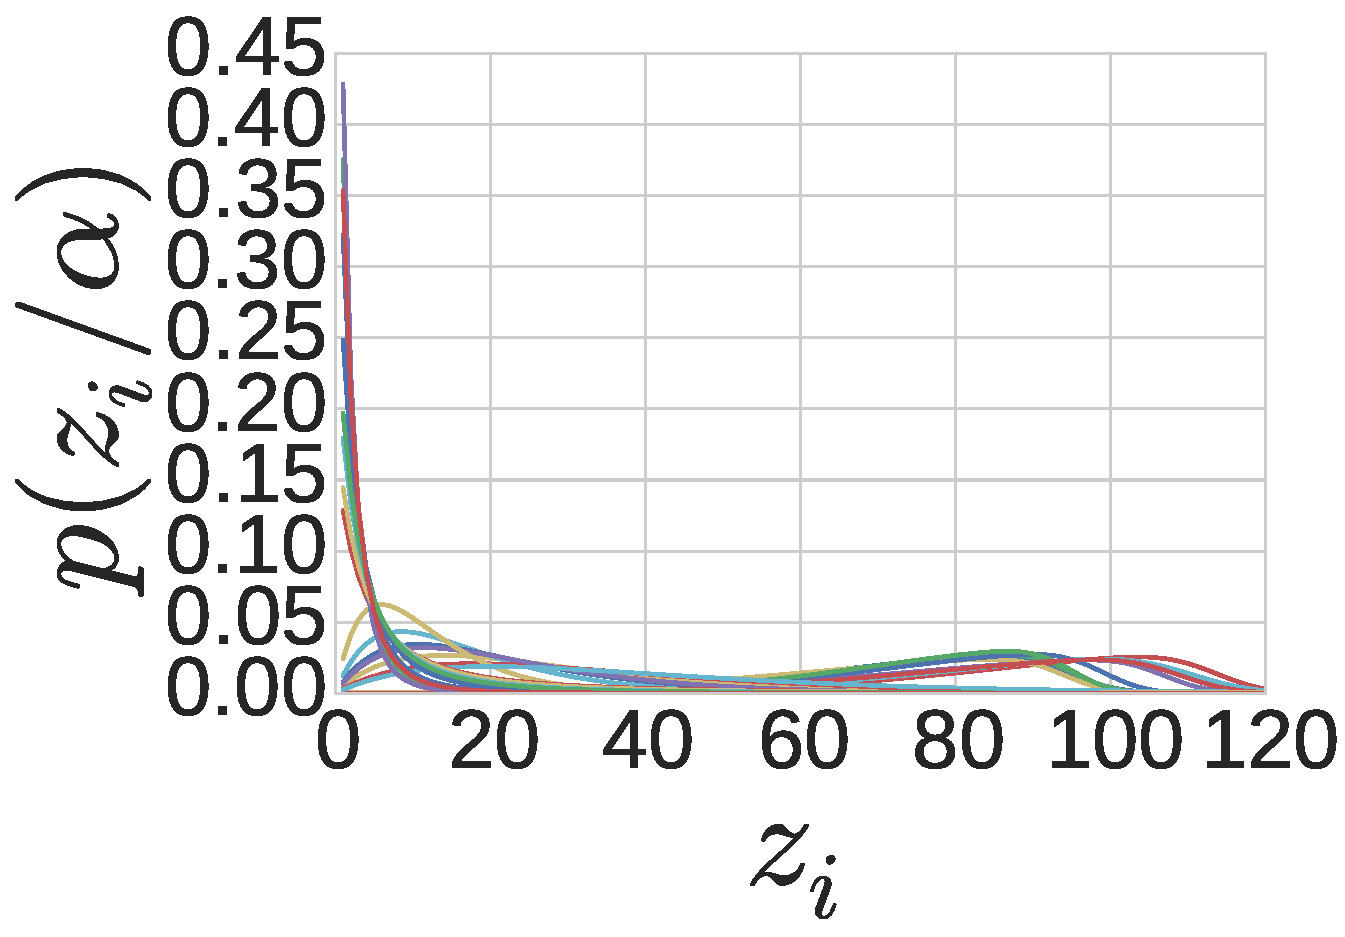
\includegraphics[width=\linewidth]{prior_full27.pdf}
        \label{fig:prior_full27}
    \end{subfigure}
    \begin{subfigure}{.24\textwidth}
        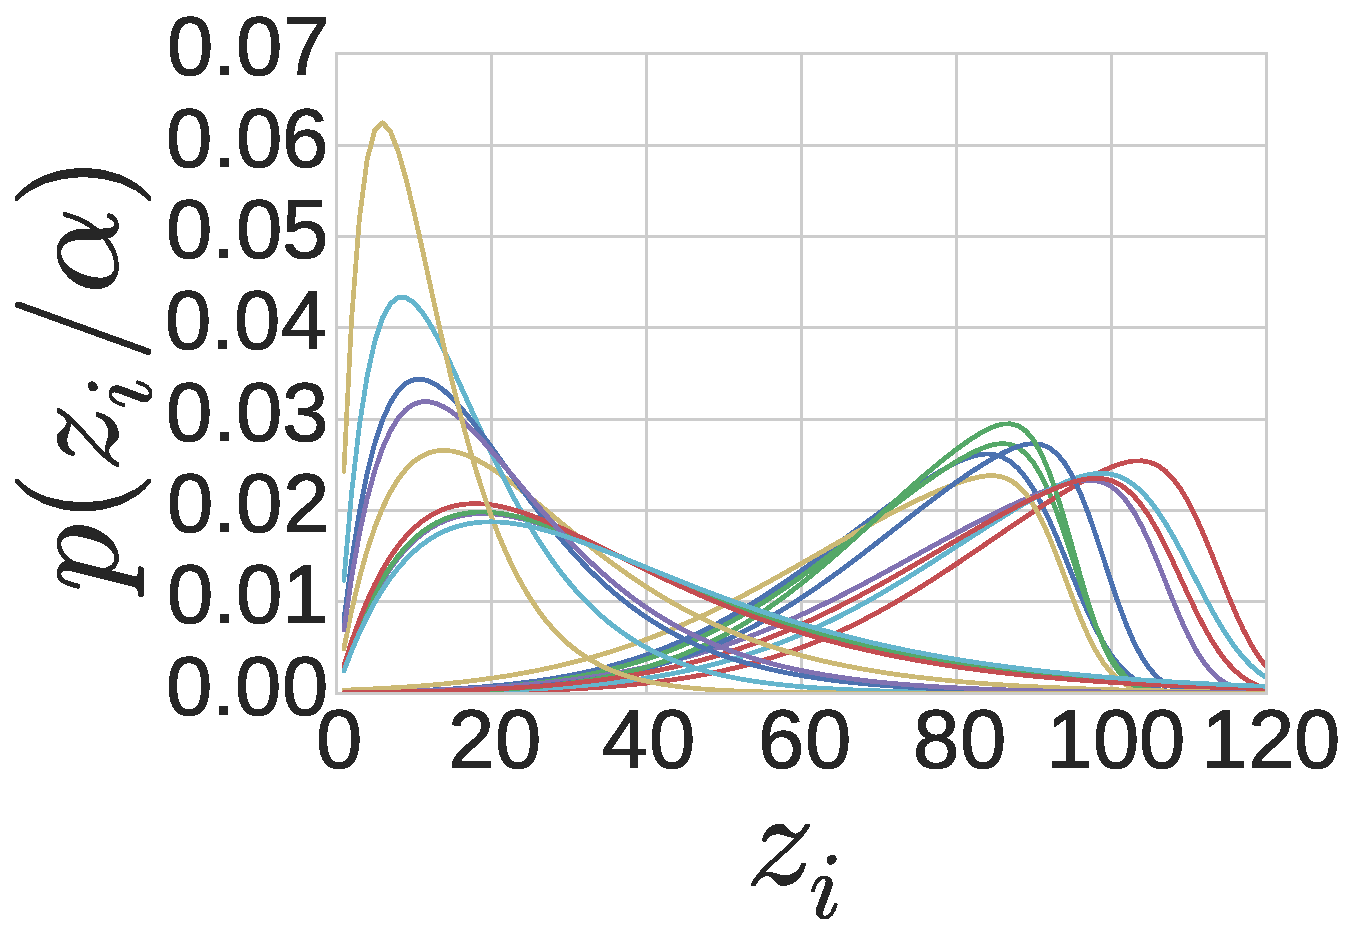
\includegraphics[width=\linewidth]{prior_partial27.pdf} 
        \label{fig:prior_partial27}
    \end{subfigure}
    \begin{subfigure}{.24\textwidth}
        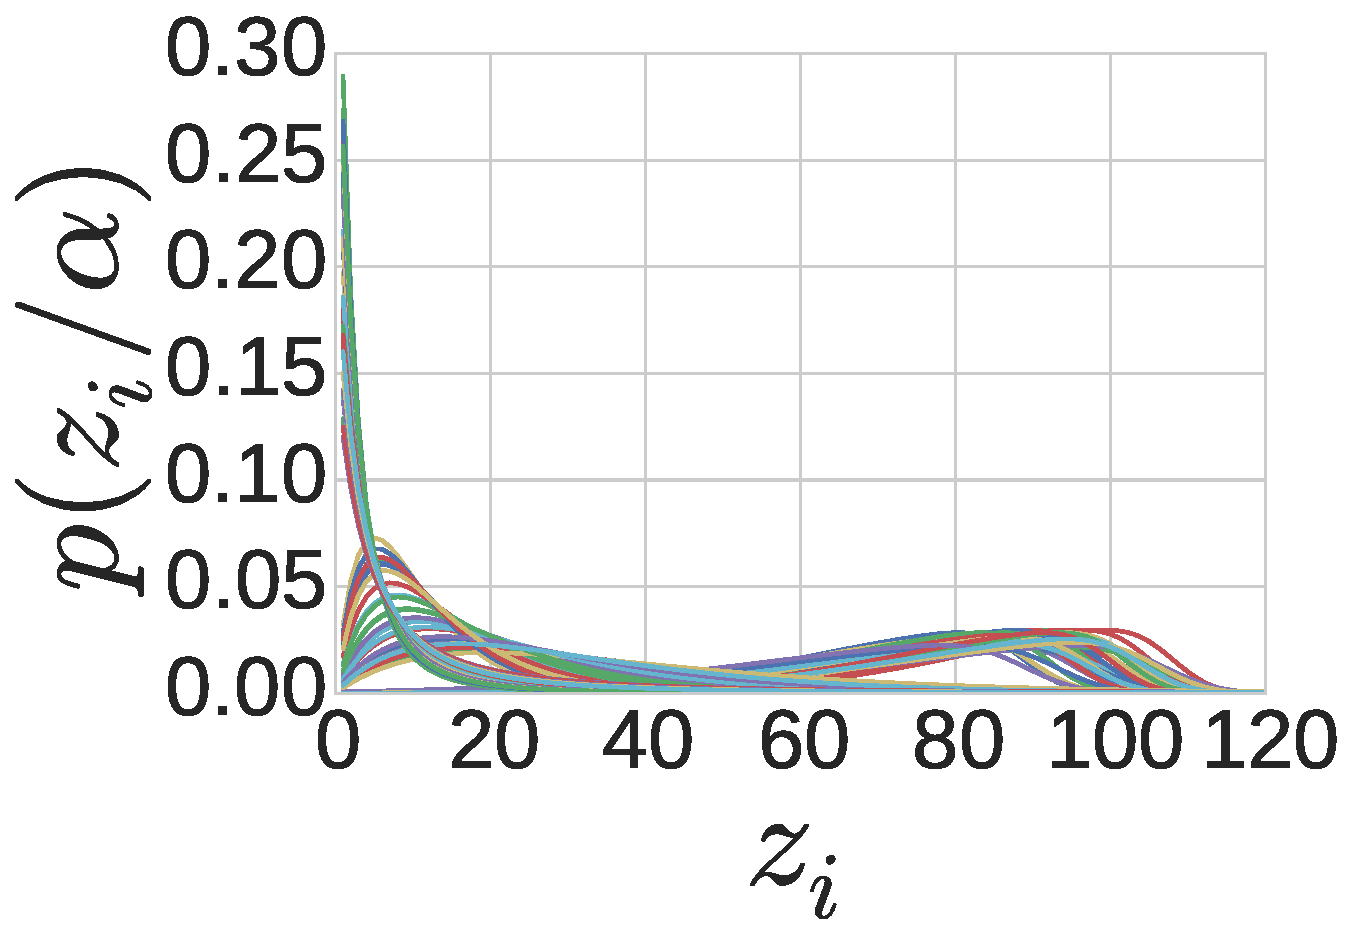
\includegraphics[width=\linewidth]{prior_full108.pdf}
        \label{fig:prior_full108}
    \end{subfigure}
    \begin{subfigure}{.24\textwidth}
        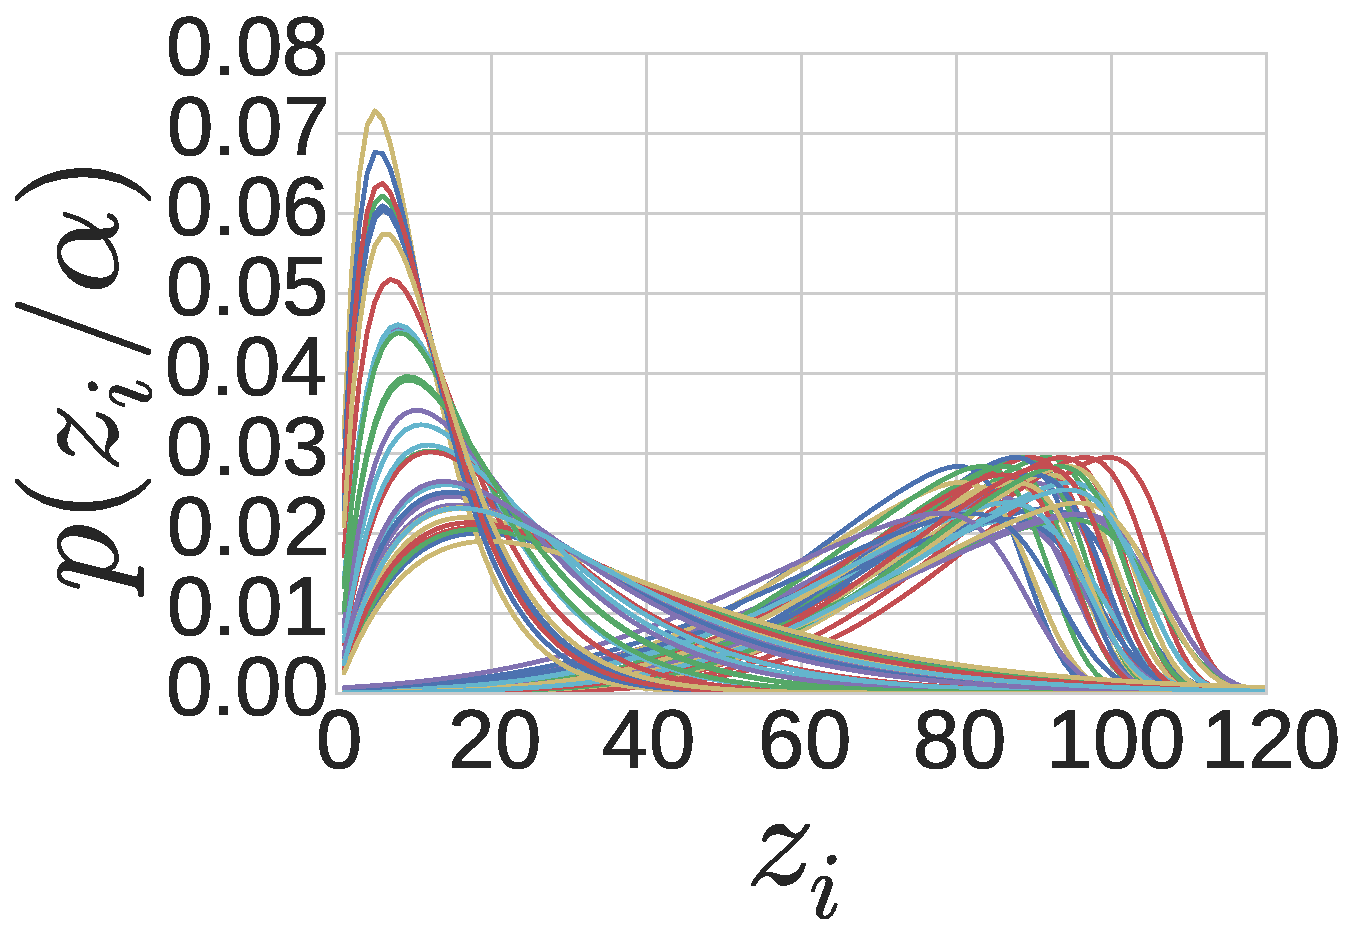
\includegraphics[width=\linewidth]{prior_partial108.pdf} 
        \label{fig:prior_partial108}
    \end{subfigure}
    \caption{(a) Prior space with $M = 27$. (b) Prior space with $M = 27$, showing only Gaussian and Erlang families for clarity. (c) Prior space with $M = 108$. (d) Prior space with $M = 108$, showing only Gaussian and Erlang families for clarity.
    }\label{fig:prior_space}
\end{figure*}

Figure~\ref{fig:model_schematic} shows the architecture of the neural model built using the Nengo neural simulator~\cite{bekolay2014nengo} based on the NEF. 

\subsection{The Neural Engineering Framework}
The NEF provides methods for implementing algorithms on vector spaces in spiking neural networks. There are three key components to the NEF. First, it describes how a population of neurons (ensemble) can form a distributed representation of time-varying vectors through non-linear encoding and weighted linear decoding. Equation~\ref{eqn:encoding} states how a vector $\vec{x}(t)$ is encoded by an ensemble of neurons. 

\begin{equation}
\label{eqn:encoding}
\begin{aligned}
a_i(\vec{x}) &= \lif{i}{J_i(\vec{x})}, \\
J_i(\vec{x}) &= \alpha_i \dotp{\vec{e}_i}{\vec{x}}{n} + J_i^{bias}
\end{aligned}
\end{equation}

Here $\lif{i}{\cdot}$ is the non-linearity that describes the neuron's spiking response,  $J_i(\vec{x})$ is the current entering the soma of the neuron, $\alpha_i$ is a gain and conversion factor, $\vec{x}$ is the stimulus vector to be encoded, $\vec{e}_i$ is the preferred direction or encoding vector and $J_i^{bias}$ is the bias current that accounts for background activity.

For this model, we choose $\lif{i}{\cdot}$ to be the leaky integrate-and-fire~(LIF) neuron model. The spiking neural model produces a spike train $\sum_m \delta(t-t_{i,m})$, where $t_{i,m}$ is the time of spike $m$ from neurons $i$. To decode an encoded vector from the activity of the neurons, the spikes are convolved with a low pass filter (to account for the post synaptic response of receiving neurons), and then weighted by linear decoding weights ($\vec{d}_i$). The decoded value $\hat{\vec{x}}(t)$ is then given by

\begin{equation}
\label{eqn:temp_decoding}
\begin{aligned}
\delta(t-t_{im}) &= \lif{i}{\alpha_i \dotp{\vec{e}_i}{\vec{x}}{n} + J_i^{bias}} \\
a_i(t) &= \sum_m h_i(t) \ast \delta(t-t_m) = \sum_m h_i(t-t_m) , \\
\hat{\vec{x}}(t) &= \sum_{i,m} h_i(t-t_m) \vec{d}_i 
\end{aligned}
\end{equation}

Second, given the encoding and decoding of vectors as described above, NEF defines how connections between ensembles can implement transformations and computations on these vectors. When two ensembles are connected, the synaptic weight matrix is given by $\omega_{ij} = \alpha_j \vec{e}_j \vec{d}_i^{f(\vec{x})}$, where $i$ indexes the presynaptic population, $j$ indexes the postsynaptic population, and $\vec{d}_i^{f(\vec{x})}$ are representational or transformational decoders. In a communication channel, representation decoders $\vec{d}_i$ are computed by the least squares optimization ${\langle||\hat{\vec{x}}-{\vec{x}}||\rangle}_x$. To perform a transformation $f(\vec{x})$, instead of finding the representational decoders we can find the transformational decoders $\vec{d}_i^{f(\vec{x})}$ by using least-squares optimization to minimize the difference between the decoded estimate of $f(\vec{x})$ and the actual $f(\vec{x})$ given by ${\langle||\hat{\vec{x}}-{f(\vec{x})}||\rangle}_x$.

Third, the NEF provides a method for directly converting any set of differential equations into a spiking network approximation of the dynamics described by those equations~\cite{eliasmith2003neural}. Specifically, the values represented by ensembles with recurrent connections can be considered as state variables in a dynamical system. The equations governing the dynamics of such neurobiological systems can be designed and analyzed using control theory methods, and translated into neural circuitry using the NEF. 


\subsection{Training data}
The model receives one observed age $x_i$ as input at a time. It uses this observation to estimate the prior over the total lifespans of people, and keeps iterating to improve the estimate until the next observation is received as input. As it receives more observations, it interpolates between the current observation and statistics from previous observations (stored in memory) to estimate the optimal prior. 

The observations $x_i$ used to train the model are generated using a two-stage hierarchical Bayes model. In particular, we generate the data in the forward direction ($\alpha \longrightarrow Z \longrightarrow X$), where $\alpha$ are the set of hyperparameters on which the true prior is conditioned. We draw a random sample $z_i$ (total lifespan of a person) from the true distribution. Each $x_i$ is drawn conditionally from $z_i$. We model $x_i|z_i \sim \mathcal{U}[0, z_i)$, meaning that we are equally likely to see a person at any time throughout their life (Equation~\ref{uniform_prob}).

\subsection{Prior space}

%We assume that rather than learning from scratch, our brain can take advantage of knowledge coming from previously learned properties of the world. 

We assume that rather than learning completely from scratch, given either evolutionary history, or personal history, or most likely a combination of both, our brain has a characterization of the set of priors most likely to capture real-world data. Thus, we assume a set of prior distributions defined as a prior space of size $M$. These distributions belong to three different families - Gaussian, Erlang and Power Law and the task is to estimate which one of them is the prior corresponding to the total lifespans. Note that these three families of distributions were chosen due to psychological evidence presented by ~\citeA{griffiths2006optimal} where they suggest that the prior beliefs informing people's predictions on a variety of tasks follow these distributions. Some of these tasks include predicting lifespans, poem lengths, movie grosses, pharaohs' reigns, etc. Thus our model can also be used to learn the priors for any of these tasks. In short we suggest a general approach that is applicable to any problem that requires estimating the upper limit of a numerical quantity given a sample drawn from that interval.

To construct the prior space, we randomly sample the hyperparameters of the distributions from a range chosen based on the psychological evidence presented by ~\citeA{griffiths2006optimal}. A skewed form of the Gaussian distribution having three hyperparameters was used with ranges: mean (89, 109), scale (5, 20) and shape (-8, -4). The Power law distribution has a single hyperparameter: shape($\gamma$) (1, 5). The Erlang distribution has two hyperparameters: scale ($\beta$) (25, 35) and shape fixed at 2.0 following~\citeA{griffiths2006optimal} and ~\citeA{shepard1987toward}. We use equal number of distributions from each family to construct the prior space. In other words, for a prior space of size $M$, the number of distributions belonging to each family is $M/3$.

\subsection{Model} 

\begin{figure*}[h]
%\setlength{\abovecaptionskip}{-3pt}
%\setlength{\belowcaptionskip}{-5pt}
    \centering
    \begin{subfigure}{.43\textwidth}
        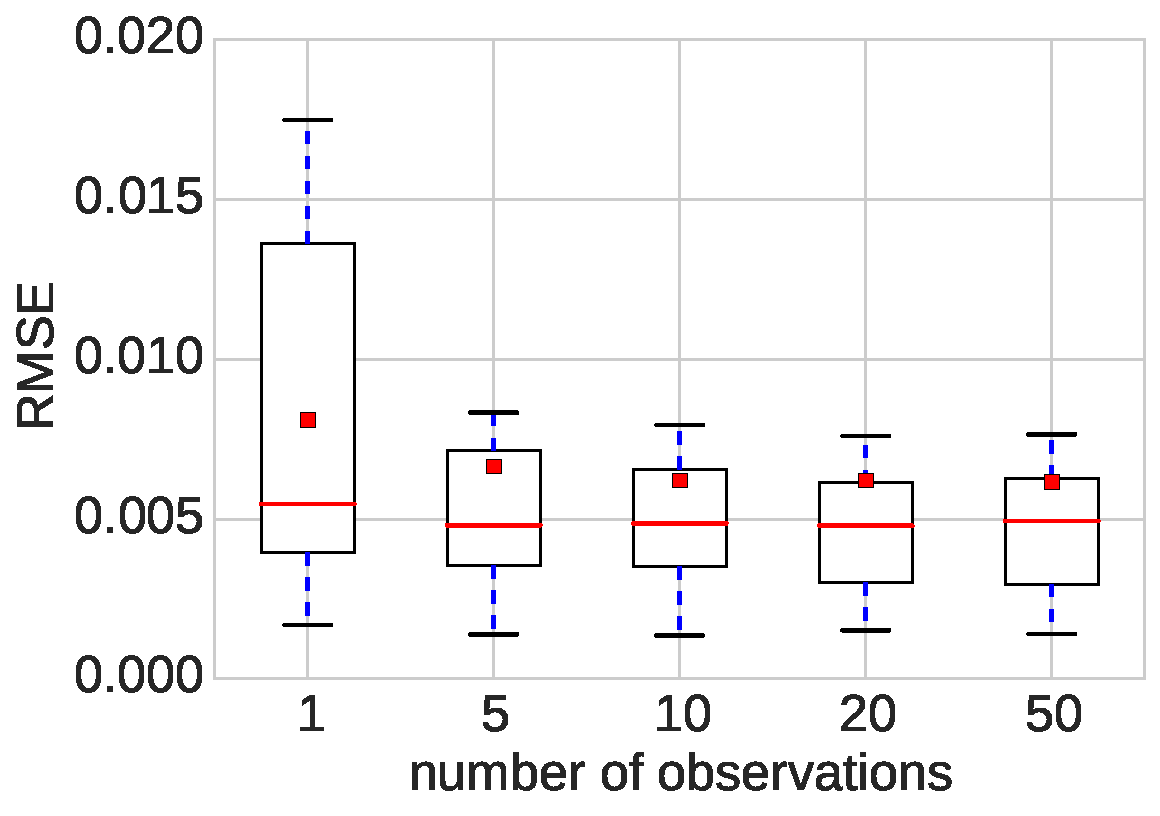
\includegraphics[width=\linewidth]{gauss27.pdf}
        \label{fig:gauss27}
    \end{subfigure}
    \begin{subfigure}{.43\textwidth}
        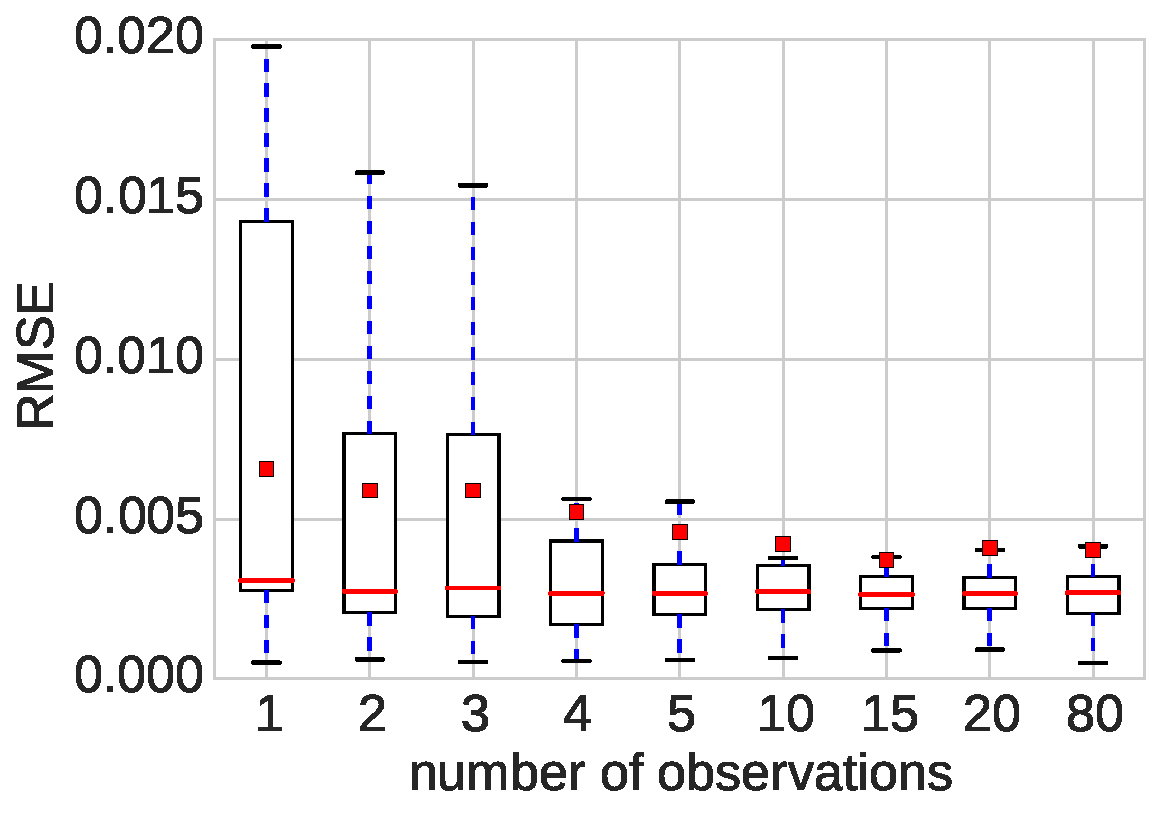
\includegraphics[width=\linewidth]{gauss108.pdf} 
        \label{fig:gauss108}
    \end{subfigure}
    \caption{Results from the neural model when a skewed Gaussian distribution is the true prior. The y-axis shows the root mean squared error relative to the true prior and the x-axis shows the number of observations used for training the model. The red squares show the mean and the red bar shows the median of the RMSE data from 100 trials.(a) Prior space of size $M=27$. (b) Prior space of size $M=108$. 
    }\label{fig:results_gauss}
\end{figure*}


As shown in Figure~\ref{fig:model_schematic}, the \texttt{sensory} node receives input and computes $T(x_i, z_i) * n_{k}$ using Equation~\ref{eqn:gb_likelihood}. It uses a random initial guess for the prior (or $\alpha^{(t)}$) to compute $p(Z | \alpha^{(t)})$ and the current input observation $x_i$ to compute $p(x_i | Z)$ (120 dimensional). We assume 120 possible values of total lifespans $z_i = \{1, 2, ..120\}$. Note that the 'node' object in Nengo does not contain neurons and performs computations mathematically. However, this computation has been abstracted only for simplification purposes and can easily be realized using spiking neurons as shown before~\cite{sharma2017}. 

The connection from \texttt{sensory} node to \texttt{cortical1} ensemble computes the transform $\log(p(Z | A))$ ($120 * M$ dimensional weight matrix). This transform contains $M$ distinct distributions defining the prior space with each distribution being 120 dimensional. This input to \texttt{cortical1} is thus $M$ dimensional where each dimension represents the utility of the corresponding prior in the prior space based on the current observation ($n_{k}s'_{i}$ from Equation~\ref{eqn:onlineEM}). The other input to \texttt{cortical1} is feedback from the Memory network, which provides utilities based on statistics of the previous observations ($(1-n_{k}) \mu$ from Equation~\ref{eqn:onlineEM}). Thus, \texttt{cortical1} represents $\mu$ and also sends it to the Memory network in each iteration for future use.

The Memory network consists of two gated difference integrator units as shown in Figure~\ref{fig:model_schematic}. Each unit consists of two neural populations per dimension, a primary population \texttt{integrator} and a \texttt{gate}. Input to the unit is given through \texttt{gate} ensemble which also receives the negative currently stored value. Thus the input to \texttt{integrator} ensemble is the difference of the current value and the target value. The \texttt{gate} ensemble can also be inhibited to disable any input to the integrator. Without any input, a recurrent connection with a long synaptic time constant ($\tau = 0.1s$) ensures that the currently stored value doesn't change much over time (except for a small drift due to noise). The two units are gated out of phase such that when the first unit is open (receives input from \texttt{cortical1}), the second unit is closed and sends it's stored value to \texttt{cortical1} in order to add the summary statistics from previous observations to the current utilities. Thus, the first unit gets the updated summary statistics as input. Next, first unit closes and the second opens to shift the summary statistics to the second unit for the next iteration.


The other output connection from \texttt{cortical1} provides input to a Winner Take All (WTA) network which is used to implement the $argmax(\mu)$ operation in Equation~\ref{eqn:onlineEM}. The WTA network that we use is called the Independent Accumulator (IA)~\cite{gosmann2017a}. It is a two-layer spiking neural network as shown in Figure~\ref{fig:model_schematic}. The first layer consists of $M$ separate integrator populations for accumulating each input, and the second layer consists of $M$ non-recurrent thresholding populations that receive one-to-one input from the first layer. The largest input accumulates the fastest, and once it reaches the threshold, it self excites and inhibits the accumulators corresponding to all other inputs. The output connection from the WTA network computes the transform $p(Z | A)$ ($120 * M$ dimensional weight matrix) which results in the current optimal prior distribution. This 120 dimensional prior is then compressed to a 20 dimensional space by computing basis $\phi_{20}(\upsilon)$ using the methods described earlier and detailed in~\cite{sharma2017}. This provides for an efficient neural representation of the high dimensional distribution in a 20 dimensional \texttt{cortical2} ensemble. The output from \texttt{cortical2} (current optimal prior) is then combined with the incoming sensory observations to continue this iterative process. 



\section{Results}

We use a skewed Gaussian distribution (the true prior for the total lifespans) to generate the observations $x_i$ for training our model. We test our model with two different prior spaces of sizes $M=27$ and $M=108$, each containing equal number of distributions from the three families - skewed Gaussian, Erlang and Power Law. We evaluate model performance by computing the root mean squared error (RMSE) of the optimal prior to which the model converges, to the true prior distribution. Both prior spaces contain distributions with RMSE ranging from 0 to 0.05. Figure~\ref{fig:rmse} shows some of the distributions to which the model converges during training. This is just meant to graphically clarify the implication of different RMSE values relative to the true distribution. 

Figures~\ref{fig:prior_space}(a, b) show the prior space of size $M=27$. Figure~\ref{fig:results_gauss}a shows the results obtained from the neural model when this prior space is used. With only one observation, the model converges to prior distributions with RMSE as high as 0.017. This implies that 25-50\% of trails converge to Erlang priors instead of the true Gaussian prior. However, with just a few more observations, the model always converges to distributions with RMSE lower than 0.007 implying that it converges to some Gaussian distribution close to the optimal. On further increasing the number of observations, there is only a slight improvement.  

\begin{figure}[ht]
\setlength{\belowcaptionskip}{-10pt}
\setlength{\abovecaptionskip}{-5pt}
\begin{center}
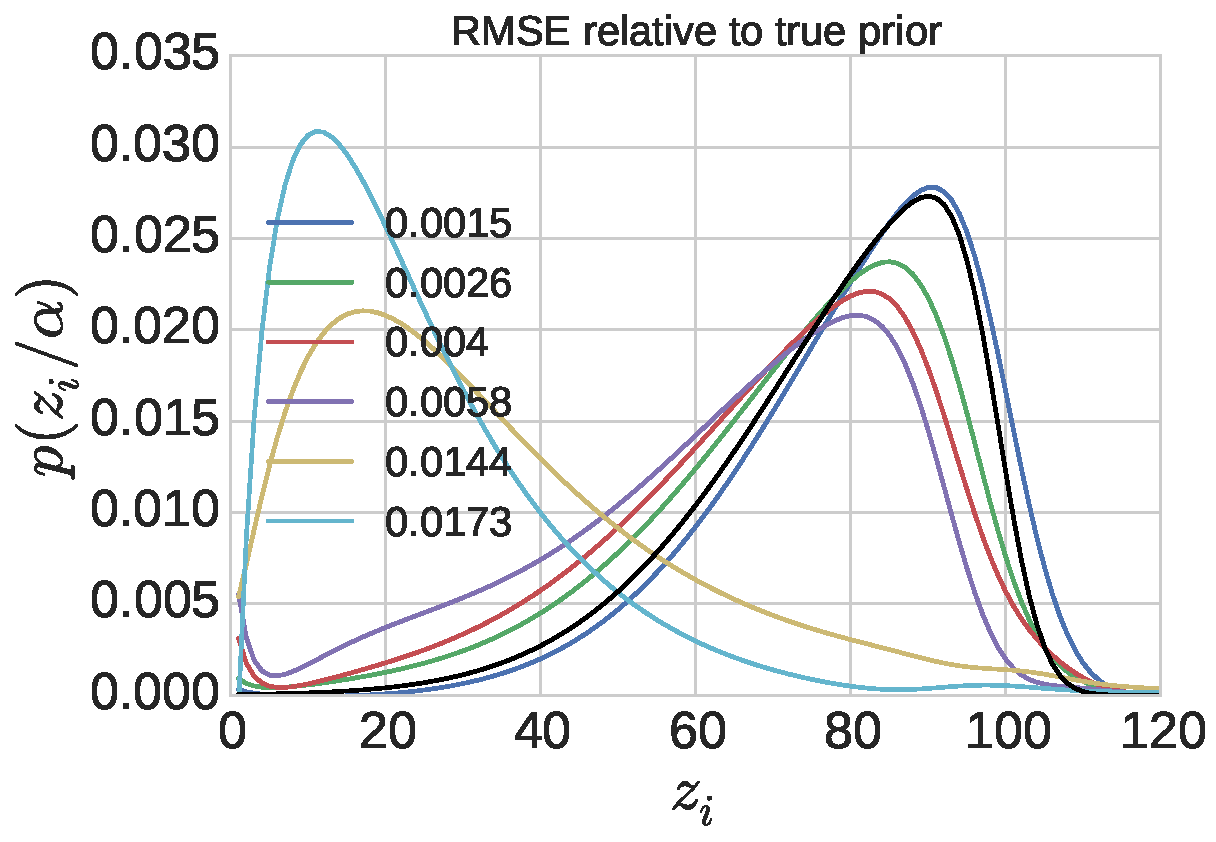
\includegraphics[width=\linewidth,keepaspectratio]{RMSE.pdf}
\end{center}
\caption{Root mean squared error (RMSE) of distributions relative to the true prior (shown in black). Power Law distributions (not shown) have RMSE ranging from 0.03 to 0.05 relative to this prior.} 
\label{fig:rmse}
\end{figure}

Figures~\ref{fig:prior_space}(a, b) show the prior space of size $M=108$ and Figure~\ref{fig:results_gauss}b shows the results obtained when this prior space is used. In this case, the initial spread of errors is even higher (upto 0.020).  This is expected due to the increase in the size of the search space. The high error implies convergence of some trials to Erlang and Power Law distributions instead of the true Gaussian prior. However, with an increase in the number of observations, the mean RMSE decreases and quickly stabilizes after around 10 observations. Interestingly, given enough observations, the model performs better with the larger prior space ($M=108$) as compared to the smaller prior space ($M=27$). In particular, with 10 or more observations, 50\% of the trials have RMSE lower than 0.0025 and the rest are still lower than around 0.0035. These distributions are very close to the optimal prior as can be judged from Figure~\ref{fig:rmse}. This performance improvement is because a bigger prior space tends to be denser and thus allows for easier navigation through the search space, by preventing the model from getting stuck in local maxima. On the other hand, a smaller prior space is sparse and more prone to getting stuck in the local maxima. 

However, an increase in the prior space size also leads to an increase in the number of neurons required for the model. In general, number of neurons scale linearly with prior space size ($M$), and are given by: $460*M + 200$. One area for future work is to explore whether this scaling can be further improved by applying the same methods of dimensionality reduction which we use to represent the optimal prior in \texttt{cortical2} ensemble in our model. The $M$ dimensional utilities represented by \texttt{cortical1} ensemble can be treated as a high dimensional vector and we can compute a basis space to compress it to a low dimensional space. This would mean that the number of neurons required for \texttt{cortical1} and Memory network would be significantly reduced, similar to \texttt{cortical2}. This compressed representation can then be reconstructed before input to the WTA network.  





%\begin{figure}[ht]
%\begin{center}
%\includegraphics[width=\linewidth,keepaspectratio]{scaling.pdf}
%\end{center}
%\caption{Plot showing the scaling of the number of neurons in the neural model with the prior space size.} 
%\label{fig:scaling}
%\end{figure}



\section{Conclusions}

%Relation to SPA??
%The ability to combine background knowledge about the world with continuous updating is critical in many aspects of higher-level cognition. 

We have presented a spiking neural network that is able to effectively learn the priors required to perform Bayesian inference in a biologically plausible way.  We constructed the network using the NEF to map the proposed algorithm to neural circuitry required for approximating the iterative learning procedure. The neural model we suggest for learning the prior for the life span inference task is generalizable to other psychological tasks (any distribution in the prior space can be the true distribution). Once we have an estimate of the prior, it can be used directly by the previously described model~\cite{sharma2017} to provide a good prediction. It is also possible to run both the prior optimization and inference at the same time and both will become progressively more accurate over time. \newline \textbf{Notes} \hspace{0.3cm} The source code for simulations and data analysis is available at https://github.com/ctn-waterloo/cogsci17-infer.


\section{Acknowledgments}
This work was supported by CFI and OIT infrastructure funding, the Canada Research Chairs program, NSERC Discovery grant 261453, ONR grant N000141310419, AFOSR grant FA8655-13-1-3084, OGS, and NSERC CGS-D.

\bibliographystyle{apacite}

\setlength{\bibleftmargin}{.125in}
\setlength{\bibindent}{-\bibleftmargin}

\bibliography{CogSci_Template}


\end{document}
